\documentclass[a4paper, 10pt]{article}

\usepackage[utf8x]{inputenc}
\usepackage[english]{babel}
\usepackage{fancyhdr}
\usepackage{hyperref}
\usepackage{url}
\usepackage{graphicx}
\usepackage{ku-forside}
\usepackage{xcolor, colortbl}
%\usepackage{cite}
\usepackage{url, hyperref}
\usepackage{amsmath}
\usepackage[numbers]{natbib}
\usepackage{listings}
\usepackage{courier}

%\setlength\parskip{1em}
%\setlength{\parindent}{0pt}
\def\arraystretch{2}

\fancyhead[LO,RE]{SmlCL \\ }
\fancyhead[LE,RO]{Philip Munksgaard \\ \today}
\pagestyle{fancy}

\titel{SmlCL}
\undertitel{An ML library for utilizing parallel architectures using OpenCL}
\opgave{Bachelorprojekt}
\forfatter{\shortstack[l]{P. Munksgaard (240789)}}
\dato{\today}
\vejleder{M. Elsman}

\newcommand{\conc}{\, \| \,}
\newcommand{\how}[1]{\text{[#1]}}

\definecolor{mygreen}{rgb}{0,0.6,0}
\definecolor{mygray}{rgb}{0.5,0.5,0.5}
\definecolor{mymauve}{rgb}{0.58,0,0.82}

\lstset{
  basicstyle=\footnotesize\ttfamily, % Standardschrift
  numbers=left,               % Ort der Zeilennummern
  numberstyle=\tiny\color{mygray},% Stil der Zeilennummern
  %stepnumber=2,               % Abstand zwischen den Zeilennummern
  numbersep=5pt,              % Abstand der Nummern zum Text
  tabsize=2,                  % Groesse von Tabs
  extendedchars=true,         %
  breaklines=true,            % Zeilen werden Umgebrochen
  breakatwhitespace=true,
  commentstyle=\color{mygreen},    % comment style
  keywordstyle=\color{blue},       % keyword style
  rulecolor=\color{black},
  stringstyle=\color{mymauve},     % string literal style
  %         keywordstyle=\color{red},
  frame=L,
  %        keywordstyle=[1]\textbf,    % Stil der Keywords
  %        keywordstyle=[2]\textbf,    %
  %        keywordstyle=[3]\textbf,    %
  %        keywordstyle=[4]\textbf,   \sqrt{\sqrt{}} %
  stringstyle=\color{red}\ttfamily, % Farbe der String
  showspaces=false,           % Leerzeichen anzeigen ?
  showtabs=false,             % Tabs anzeigen ?
  xleftmargin=17pt,
  framexleftmargin=17pt,
  framexrightmargin=5pt,
  framexbottommargin=4pt,
  %backgroundcolor=\color{lightgray},
  showstringspaces=false,      % Leerzeichen in Strings anzeigen ?
  captionpos=b
}

\begin{document}
\maketitle
\newpage
\tableofcontents
\newpage

\section{Introduction}


\section{Problem Description From Synopsis}

In this project \emph{I want to examine whether or not it is possible
  to construct a Standard ML library for utilizing parallel
  architectures using OpenCL, that will enable users to achieve
  significant speedups in potentially parallel computations compared
  to traditional sequential architectures}.


\section{Motivation}


\section{Parallel Computing, the GPU Architecture and OpenCL}

As CPU clock speeds started to reach an upper bound of feasibility in
about 2004~\cite{clockspeed}, processor manufacturers started to look
for new ways to increase the speed of computation in
computers. Parallelization quickly proved to offer speedups in form of
parallel computations. The idea is simple: use two or more cores in
parallel to work on different aspects of a problem and merge the
results in an effective manner.

As an example, suppose that we want to increment all elements in an
array of $n$ integers by one. Using a traditional CPU would require
$n$ sequential operations on the array, but if two traditional CPUs
could somehow share the memory between them, then one of the CPUs
could process one half of the array, while the other CPU processes the
other half at the same time. We still require $n$ operations on the
array, but it only takes half the time.

\subsection{Parallel architectures}

Of course, many different parallel architectures exist, with
individual scales and applications.

\emph{Grid computing systems}, where computation takes places across
multiple independent administrative domains, offer the largest scale
of parallel computing. Typically, grids, as they are also called, are
comprised of many different devices owned by seperate entities, who
pool their resources together. A famous example of grid computing is
the SETI@home project~\cite{seti}, where hundreds of thousands of
people around the globe connect over the internet to volunteer their
computer resources towards the search for extraterrestrial
life~\cite{seti-number}. The project has since spawned the BOINC
grid-computing framework, which is used to research things like
protein folding \cite{boinc-other} using the same techniques. These
systems offer massive computational power, at the cost of low speed of
transfer, as well as the need to have a central server delegate
sub-tasks to the individual participants in the grid. As a result of
the low speed of transfer, the sub-tasks must be relatively
independent, and require a high-time-of-computation to data-size
ratio, for grids to be efficient.

\emph{MMP (Massively Parallel Processor) systems}, commonly associated
with supercomputers, frequently take up entire storage
facilities~\cite{supercomputer-size}, and are composed of thousands of
processors connected via highly specialized interfaces that have been
constructed specifically for the purpose of the supercomputer. They
typically offer very high computational power, much better
communication between processors than grids, but at an enormous
cost~\cite{supercomputer-cost}. These machines are typically owned by
government institutions and agencies, and are used for research, in
the military, as well as in meteorological
computations~\cite{supercomputer-use}.

\emph{Cluster server systems}, are composed of multiple general
purpose computers that share computational resources and data across a
specialized network. Typically used for application servers in
businesses~\cite{clusters-in-business}, they are not quite as
expensive as supercomputers, but provide a significant boost in power
compared to traditional servers, as well as the ability to provide
redundancy and fail-over services.

\emph{Symmetric multiprocessing (SMP) systems}, are traditional
computers containing multiple identical processors connected as a
single unit~\cite{smp}. Examples of these include Intel Core 2 Duo
processors, which is actually comprised of two Intel Core 2 processors
acting in unison~\cite{intelcore2duo}. Some of the first experiments
with parallel architectures for consumer PCs are examples of SMP
systems. In fact, at a certain point, some motherboards had two CPU
sockets, allowing the user to install an additional identical CPU for
a speed boost~\cite{two-cpus}.

\emph{Multi-core processors}, consist of a single chip with more than
one computing core. Many modern CPUs contain more than a single core,
the Intel Core 2 processor, for example, contains 2~\cite{intelcore2},
but multi-core processors are commonly associated with video
cards. Video cards include one or more \emph{GPUs (Graphical
  Processing Units)}, which is a multi-core processor specifically
designed for certain parallel kinds of operations pertaining to
graphics processing. Originally designed and sold to consumers to
enhance 3-D graphics in video games, because of their parallel
architecture, GPUs have since found many other applications.

\subsection{Graphical Processing Units}

Modern GPUs include hundreds or thousands of cores that all can be
used in parallel to effectively perform such things as matrix
operations and operations on large arrays; when it comes to these
kinds of operations GPUs offer huge speed gains compared to
traditional CPUs, at an affordable price.

GPU architectures, such as NVIDIAs Kepler GK110, typically consist of
a number of cores, grouped in some number of groups. On top of an
amount of shared memory between all groups, each group has its own
memory, that all cores in the group can uniformly access.

\begin{figure}
  \centering
  \caption{Diagram of NVIDIAs Kepler GK110 architecture}
  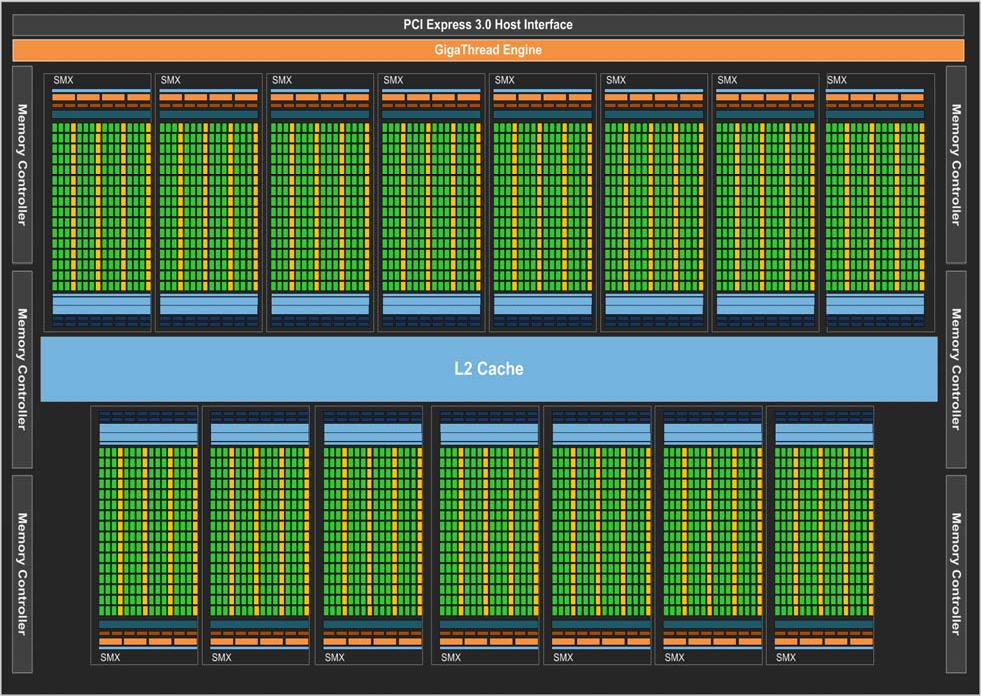
\includegraphics[width=1\textwidth]{figures/kepler110.png}
  \label{kepler}
\end{figure}

As an example, the Kepler GK110 is equipped with 15 groups of cores,
called \emph{Streaming Multiprocessors (SMX)}, each with 192
single-precision cores, and 64 double-precision cores and several
other cores for more specific operations~\cite{kepler}. Each streaming
multiprocessor has 64 KB of memory that is shared between its cores,
in addition to 1536 KB memory that is shared between all of the
streaming multiprocessors.

In order to efficiently take advantage of all this parallel processing
power, special care must be taken when programming for the GPU. We
have to efficiently divide the work into parts, distribute them across
groups and cores, make sure that cores do not overwrite the work of
each other, synchronize results and so on. Luckily, frameworks, such
as \emph{OpenCL}, can help us with these tasks.

\subsection{OpenCL}

Originally created by the non-profit technology consortium Khronos
Group~\cite{khronos}, and since embraced by numerous hardware and
software companies, including AMD and NVIDIA, the two biggest
manufacturers of GPUs, OpenCL is ``a framework suited for parallel
programming of heterogeneous systems''~\cite{opencl-quote}. With it,
you can write programs that runs uniformly on both CPUs and GPUs, as
well as Digital Signal Processors and other kinds processors
supporting the framework, allowing you to take advantage of many
different architectures using the same code.

In OpenCL, programs are made up of \emph{kernels}, which are written
in a C-like language and some host code. Each kernel takes a set of
arguments, performs some kind of computation, and modifies one or more
of the arguments to include the result (in OpenCL, kernels cannot
return values, therefore results are returned to the caller via
in-memory data-structures). \emph{Work groups} are made up of a number
of kernels, and arguments to kernels can be either global (all kernels
access the same memory), local (only kernels in the same work group
can access the same memory) or private (no other kernel can access
this memory). Each kernel also has a unique global ID, a work group
ID, and a unique ID within it's work group.

The host code, typically written in C or C++~\cite{hostlang}, uses the
OpenCL API to set up the OpenCL environment, select a device to ,
compile and build the kernel code, transfer data to buffers on the
device, execute the kernels and read the results back from the
buffers. Appendix \ref{vectoradd}, shows the code required to
calculate the addition of two vectors.


\section{Interfacing with OpenCL from ML}

We want to facilitate an easy and safe way to take advantage of the
computational power of GPUs. By hiding some of the complexities of
parallel computations and choosing some sane default options, we hope
to make a simple interface to OpenCL that is easily usable from
Standard ML, without divulging too much of OpenCLs internal workings.

In order to achieve this, we have built a series of abstraction layers
on top of OpenCL: \emph{SimpleCL} is a C library that provides a
simplified API to OpenCL, the first iteration of \emph{Smlcl} then
provided a dumb interface from \emph{MLton}, an implementation of Standard
ML, to SimpleCL. Building on top of Smlcl, we've added the ability to
safely generated typed kernels and execute them in a type safe manner.

\subsection{SimpleCL}


\section{Type safety and phantom types}


\section{Type Safe OpenCL Kernel Execution}

Now that we have introduced phantom types, we are ready to describe
our implementation of SmlCL.

The first iteration of the SmlCL interface provided the
following functions:

\begin{itemize}
  \item \texttt{init}: Initiates a GPU device and returns a value of
    the type \texttt{machine}, which is used to execute commands to
    the device.
  \item \texttt{Real} and \texttt{Int}: Returns a type variable of
    type \texttt{$\alpha$ T} (instantiated with the corresponding
    types), containing closures for making, reading, and writing to
    buffers.
  \item \texttt{mkKern1} and \texttt{mkKern2}: Is used to compile
    kernels from source code in the form of a text string. The
    functions are used to compile kernels that take 1 and 2 input
    buffers as arguments, respectively, in addition to an output
    buffer. No checking is done on the source string, so this function
    relies on the source string being syntactically and semantically
    correct, while relying on additional type arguments for
    determining the type of the resulting \texttt{kern1} and
    \texttt{kern2}.
  \item \texttt{mkBuf}, \texttt{readBuf}, and \texttt{writeBuf}:
    Functions for handling buffers. We can create a new buffer
    containing the elements of an input array, read the contents of a
    buffer into an array, and write the contents of an array to an
    already existing buffer (while making sure that the input array is
    no larger than the size of the buffer).
  \item \texttt{kcall1} and \texttt{kcall2}: Executes a kernel. Takes
    a number of input buffers as arguments, and produces a resulting
    output buffer. Also takes an integer, the work size \texttt{n}, as
    argument, and assumes that the output buffer contains \texttt{n}
    elements.
\end{itemize}

The implementation of SmlCL takes advantage of phantom types to
ensure that programs are well typed by making the types for buffers
and kernels parameterized. Since they can only be instantiated using
\texttt{Real} and \texttt{Int}, which have types \texttt{real T} and
\texttt{int T}, respectively, they each get the appropriate type.

The major weak points are \texttt{mkKern1} and \texttt{mkKern2}, since
they rely on the user to provide the correct types for the source
string, as well as the source string actually being correct OpenCL C.
To help alleviate this problem, SmlCL has been extended with kernel
generating facilities.


\section{OpenCL Kernel Generation}
\label{kerngen}

We wish to avoid having to code kernels in OpenCLs C-like language. In
the implementation of SmlCL that we have described so far, kernels are
simply strings that we manually attach some types to. It is easy to
see, that this approach has the potential of introducing a great many
bugs and errors in our program. Firstly, because we have no way of
knowing whether or not the source code we read from a file is actually
valid OpenCL C or not, but also because we don't know if the types
we attach to the kernels are correct.

Both of these problems can be solved by having SmlCL generate kernels
for us, which is what we have chosen to do in SmlCL.

We have extended SmlCL with the type \texttt{$\alpha$ expr}, and the
following functions for constructing expressions, where we again make
use of phantom types to guarantee that expressions are well-typed:

\begin{itemize}
  \item \texttt{IntC}: Models an integer constant.
  \item \texttt{RealC}: Models a constant of type real.
  \item \texttt{Add}, \texttt{Sub}, \texttt{Mul}, and \texttt{Div}:
    Addition, subtraction, multiplication, and division of two expressions of the same type.
  \item \texttt{Eq}, \texttt{And}, \texttt{Or}, and \texttt{Not}:
    Equality, and the boolean operations and, or, and not.
  \item \texttt{IntToReal} and \texttt{RealToInt}: Conversion between
    types.
\end{itemize}

Note that there is seemingly no way to access the buffer-arguments to
the kernel. In the structure implementing SmlCL, you can see that
there are functions \texttt{Buf1} and
\texttt{Buf2}, which take a type variable and an index (can be either
\texttt{This}, referring to the value in the buffer corresponding to
the particular instance of the kernel that is running, through
\texttt{get\_global\_id(0)}, an absolute index into the array, or an
offset from \texttt{This}), and return an expression of the given
type. If we had simply exposed these functions to the user, he would
be able to construct badly typed expression such as \texttt{Add (Buf1
  Real This) (Buf1 Int This)}. Instead, the user is required to pass a
closure to the kernel generating functions, where the arguments to the
closure correspond to specific buffers. Here is what that looks
like:

\begin{lstlisting}[mathescape,language=ML,caption=Expressing VectorAdd
  using SmlCLs expression generating capabilities.,label=vectoradd2]
  mkKern2 machine
          "VectorAdd"
          (fn (b1, b2) => Add (b1 This) (b2 This))
          (Real, Real)
          Real;
\end{lstlisting}

Where the types for the buffers is given as the fourth and fifth
argument. In this way, we are guaranteed that all references to a buffer
has the same type.

As an example of how expression generation works, here is the kernel
generated by running the code in Listing \ref{vectoradd2}:

\begin{lstlisting}[mathescape,language=C,caption=VectorAdd as
    generated by SmlCL]
  #pragma OPENCL EXTENSION cl_khr_fp64 : enable
  __kernel void VectorAdd(
  __global const int* buf1,
  __global const double* buf2,
  __global double* bufr) {
  int iGID = get_global_id(0);
  bufr[iGID] = ((real)(buf1[iGID]) + buf2[iGID]);
  }
\end{lstlisting}

As the observant reader might have noticed, currently SmlCL can only
represent a \emph{very} limited subset of C. For instance, there is no
way to represent statements and control flow structures. In their
current form, expressions are limited to a single statement, assigning
a value to the position in the buffer corresponding to the current
global id. While allowing us to keep the expression generator rather
simple, this is obviously not ideal, and, as we'll discuss in chapter
\ref{futurework}, an obvious improvement allow conditional statements
like if statements, loops, temporary variables and the like.


\section{Pre-Defined Kernels Templates in SmlCL}

Since the kernels generated using \texttt{mkKern1} and
\texttt{mkKern2}, always follow the same strict pattern where each
instance of the kernel assigns a value to its corresponding slot in
the output buffer, they have limited practical uses. For example, it
is not possible to create a kernel that sums all of the elements in an
array.

In order to allow users to perform some of the common functions on
collections of values, like map and reduce, we have extended SmlCL
with some convenience functions for common operations.

\subsection{Map}

\begin{lstlisting}[language=ML,mathescape,caption=Signature for \texttt{map}]
val map : machine $\to$ ($\alpha$ expr $\to$ $\beta$ expr) $\to$ $\alpha$ T $\to$ $\beta$ T $\to$ ($\alpha$, $\beta$)kern1
\end{lstlisting}

The \texttt{map} function is used to create a kernel that maps a
function onto a buffer in parallel, with the result ending up in a new
buffer. For example, the expression
\begin{lstlisting}[language=ML,label=mapkern,caption=Sample call to \texttt{map}]
  map m (fn x => Div (Mul x x) (RealC 1.5)) Int Int
\end{lstlisting}
will yield the following kernel
\begin{lstlisting}[language=C,label=vectoradd,caption=Resulting kernel
  from the call in listing \ref{mapkern}.]
  #pragma OPENCL EXTENSION cl_khr_fp64 : enable
  
  __kernel void map(__global double* buf1,
                    __global double* bufr) {
    int iGID = get_global_id(0);
    bufr[iGID] = ((buf1[iGID] * buf1[iGID]) / 1.5);
  }
\end{lstlisting}

As such, it is a rather straightforward implementation, and could have
been approximated by the user of SmlCL like this:

\begin{lstlisting}[language=ML,caption=Approximation of \texttt{map}
    function.]
  mkKern1 m "map" (fn x => Add (x This) (x This)) Int Int
\end{lstlisting}

Except that we then have to directly specicify which index
(\texttt{This}) into the buffer we are operating on.

Since this is a rather straightforward function, it doesn't offer a
lot of room for fine-tuning, which unfortunately also means that it is
not all that fast compared to traditional sequential code.

\begin{table}
  \center
  \label{maptable}
  \begin{tabular}{l|l}
    CPU  & GPU  \\ \hline
    5452 ms & 4500 ms \\ \hline
    5452 ms & 4496 ms \\ \hline
    6048 ms & 4780 ms \\ \hline
  \end{tabular}
  \caption{Measurements of execution time for a simple operation on
    each element of an array.}
\end{table}

Table \ref{maptable} shows three measurements of how long it took (in
milliseconds) to run the program in appendix \ref{app:map}, using the
GPU and the CPU respectively. The code performs a simple mapping like
the one in listing \ref{mapkern} a hundred times on a randomly
generated array of reals.

As we can see, the GPU code actually performs slower than the CPU
code. This is due to the fact that we have to generate the array of
random numbers on the host-side and transfer it to the GPU device
before we can even start working on it. Data-transfer is very slow
compared to data-processing, and acts as a bottle-neck for this
test. In order to achieve better performance, the GPU kernel has to be
more computationally expensive, so that the time of computation
greatly outweighs the time of transfer. A better approach would be to
generate the random numbers on the GPU device itself. Unfortunately,
the OpenCL run time does not support traditional C-like random number
generation using \texttt{rand()}. Instead, we can chose a uniform
distribution of numbers between $0$ and $1.0$ and let the kernel
generate those. This approach will be demonstrated later in chapter
\ref{sec:pi}.

\subsection{Reduce}

The \texttt{red} function is the parallel equivalent of the
traditional \texttt{reduce} function. It takes a function from $\alpha
* \beta$ to $\beta$, and iteratively applies that function to elements
of the input buffer, accumulating the results in the second parameter.

\begin{lstlisting}[language=ML,mathescape,caption=Signature for \texttt{red}.]
  val red : machine $\to$ ($\alpha$ expr * $\beta$ expr $\to$ $\beta$ expr) $\to$ $\beta$ expr $\to$ $\alpha$ T $\to$ $\beta$ T $\to$ ($\alpha$, $\beta$)kern1
\end{lstlisting}


For example \texttt{red m (Add x x) (IntC 0) b Int} where \texttt{b}
is a buffer of type \texttt{int buf}, would return the sum of all the
elements in the buffer. Note that this function, unlike map, does not
return a kernel, but immediately returns the result.

Reductions on the GPU can be done in a number of ways. The most simple
is to have a single thread iteratively go through the entire array and
calculate the reduction, but then we are just doing the reduction
sequentially and might as well do it on the CPU. Instead, we can
choose to take advantage of the associative and commutative properties
of many common reduction operations. For example, if we simply want to
calculate the sum of all elements in an array, or find the highest or
lowest value, we do not care in which order the elements are
processed. One way to take advantage of this, is to have each kernel
separately compute intermediate reductions for part of the array,
followed by a single reduction of the intermediate results. Our
reduce-kernel follows this approach, by having each kernel calculate
the reduction of part of the input array and store it in the output
buffer at the position corresponding to their global id, waiting for
all kernels to sync up, and then having the first kernel (with global
ID 0) sum up the intermediate results into the first location in the
output buffer. 

Because of the way the reduction is computed, we felt that it would be
easiest to let \texttt{red} automatically extract the result from the
output buffer, which is why it cannot simply return a kernel.

\subsection{Approximating $\pi$.}
\label{sec:pi}

We saw above that mapping a relatively simple function onto an array
using SmlCL did not yield much, if any, improvement in performance. We
are now going to focus on something a little more computationally
demanding: approximating $\pi$.

Suppose you have a circle of radius $1$ inside a square of width
$2$. The area of the circle $a_c$ is $\pi r^2 = \pi$, the area of the
square $a_s$ is $2*2=4$, and the ratio $a_c \over a_s$ is $\pi \over
4$. That means, that if we arbitrarily sample points within the
square, the chance that it is within the circle as well is $\pi \over
4$. We can even split the square up into 4 parts, representing the
quadrants in a regular graph, and since each quadrant is simply an
mirrored image of the other quadrants, we can simply sample points
within one of the quadrants estimate $\pi$. Simply put, if we randomly
select $n$ numbers $x_1, \ldots, x_n$ and $y_1, \ldots, y_n$, between
$0$ and $1$, the amount of points $(x_i, y_i)$ for which $x_i^2 +
y_i^2 \leq 1$ is approximately $\pi n \over 4$. This is called the
Monte Carlo method for $\pi$.

\begin{figure}[h]
  \center
  \caption{Sampling of points in a circle. Source: \url{http://math.fullerton.edu/mathews/n2003/montecarlopimod.html}}
  \label{fig:pi1}
  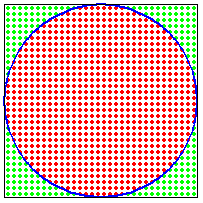
\includegraphics[scale=0.5]{figures/pi1.png}
\end{figure}

Using this knowledge, we can use the \texttt{map} and \texttt{red}
functions to estimate $\pi$. Table \ref{table:pi} shows the result of
computing $\pi$ using this method. Each simulation runs 100 times and
uses 1000000 randomly generated numbers. The source code is listed in
appendix \ref{app:pi}. 

\begin{table}
  \center
  \label{table:pi}
  \begin{tabular}{l|l}
    CPU & GPU \\ \hline
    11964 ms & 11500 ms \\ \hline
    10332 ms & 11308 ms \\ \hline
    9132 ms & 10864 ms \\ \hline
  \end{tabular}
  \caption{Estimating $\pi$ using the Monte Carlo method. The code can
  be seen in appendix \ref{app:pi}.}
\end{table}

The parallel program performs about as fast as the sequential
one. Again, this must be attributed to the high cost of transferring
data to the device, compared to the relative simple computation
taking place.

To properly take advantage of the capabilities of the GPU, it is clear
that we must minimize data transfer, and perform as much computation
on the GPU as possible. One way we could get better performance in our
benchmark above, would be to have the GPU generate the random numbers
itself. Unfortunately, the OpenCL runtime does not provide standard
\texttt{rand()} type functions. 

If we, instead of relying on random numbers, simply generate a list of
numbers from $0$ to $1$, like $0.0, 0.0, 0.1, \ldots, 1.0$, we still
get the same distribution of points inside the circle, but without the
random element. This allows us to let the kernels calculate their
points individually, and thus we avoid having to transfer a large
buffer of numbers to the device before we can start computing.

\begin{table}
  \center
  \label{table:altpi}
  \begin{tabular}{l|l}
    CPU & GPU \\ \hline
    78556 ms & 1100 ms \\ \hline
    78436 ms & 1088 ms \\ \hline
    78168 ms & 1096 ms \\ \hline
  \end{tabular}
  \caption{Estimating $\pi$ using evenly distributed
    numbers from $0$ to $1$.}
\end{table}

Unfortunately, the current expression generator functions in SmlCL are
not powerful enough to express such a kernel. Thankfully, we can use
PrimCL instead and supply it with a manually coded kernel. Table
\ref{table:altpi} shows the results of running the code in appendix
\ref{app:altpi}, showing a significant performance boost from using
the GPU compared to the CPU. This indicates that, in order to take
full advantage of the parallel architecture of the GPU, we have to
extend the SmlCLs expression generator capabilities to allow more
advanced constructions such as loops.


\section{Assessment}


\section{Future Work and Extensions}
\label{futurework}

The current implementation of SmlCL represents an initial
implementation of a Standard ML interface to OpenCL, that tries to
keep within the functional paradigms of SML, while allowing users to
take advantage of some of the capabilities of modern GPUs. While it
achieves many of its goals by being easy and safe to use, it does not
yet take full advantage of OpenCL and its capabilities, and thus there
is still plenty of room for improvements.

A relative simple addition to the current interface would be to
allow for additional types of buffers and values. Currently, SmlCL
only supports buffers and base values of type \texttt{int} and
\texttt{real} (\texttt{int} and \texttt{double} in C,
respectively). Although C does not have native support for boolean
values like \texttt{true} and \texttt{false}, it does support boolean
logic, simply by regarding the number $0$ as false, and everything
else as true.  Support for SML characters like \texttt{\#"a"} could
also be added rather easily, since for most cases they share the same
representation in Standard ML and C. Strings could also be passed
rather easily, but special care needs to be taken not to allow
any overflows, since different SML implementations have different
representations of strings (they are not null terminated in MLton, for
example). However, adding support for tuples and datatypes is not very
feasible; MLton does not even allow passing datatypes or tuples to C
functions, and it would needlessly complicate kernels as well.

Another trivial extension to SmlCL would be to add more versions of
\texttt{mkKern} and \texttt{kcall}, each allowing a different amount
of buffer arguments. One would need to add run functions to all the
layers of SmlCL, including PrimCL and SimpleCL, but the
implementations would be more or less identical to the already
existing run functions. However, a nicer approach would be leverage
the type-system to allow creations of type-parameterized kernels of
arbitrary arity, and being able to execute them with a single
function. \citet{danvy1998functional} describes a technique for
simulating C's \texttt{printf} function in Standard ML, that could be
used to implement the desired n-arity kernel calls in SmlCL.

One could also allow for static handling of buffer
sizes. By emplying the techniques demonstrated in ~\cite{buffersize}
we can statically guarantee that all kernels are called with suitably
sized buffers.

SmlCL currently only supports passing buffers as arguments to
kernels. A nice addition would be to allow users to pass regular
scalars like integers or reals. However, this poses several problems
for the implementation: firstly, we would need to extend the function
definitions of \texttt{kcall1} and \texttt{kcall2} to allow not only
buffers, but also integers and reals as arguments. Sadly, this is not
easily possible using the current way we execute functions: we would
need to add some datatypes to manage the different types of arguments,
and we would have to add a lot of foreign function calls for each
composition of argument types. Another way to achieve this would be to
refactor the code, such that we had functions like:

\begin{lstlisting}[language=ML,mathescape]
  val setArgBuf : kernel -> int -> 'a buf -> unit;
  val setArgReal : kernel -> int -> real -> unit;
  val setArgInt : kernel -> int -> int -> unit;
\end{lstlisting}

That is, we manually set the kernel arguments on the SML side, instead
of letting the C-side handle them.

We could also extend our interface to OpenCL, allowing users to
specify work-group sizes, adding support for OpenCL vectors, using
kernels that have been compiled offline, use CPUs in addition to GPUs,
and much more. OpenCL is very complex, and has many options for
customization of execution and how to run your programs. However, we
feel that many of these additions would work counter to our goals of a
simplified API that hides some of this complexity in order to provide
ease-of-use. It would however enable users to better take advantage of
the capabilities of OpenCL, and if a suitable compromise could be
found, it could facilitate more efficient parallel processing.

Finally, we could extend the expression generator, in order to allow
the construction of more complex kernels, including additional
constructions like \texttt{if}-statements, \texttt{for} and
\texttt{while} loops, auxiliary functions, global constants, local and
private variables, and so forth. This could be done in a number of
ways, one could either provide sufficient constructs such that our
expression interface mimics OpenCL C, or one could keep a functional
approach and add more constructs like \texttt{Map} and \texttt{Fold},
\texttt{Let} statements, and the like to the language. For this
project, we have chosen to keep it relatively simple, in order to make
sure that kernels execute correctly. The expression generator could
also be extended to allow for kernel composition, such that one could
be combined two or more kernels into one execution, effectively
creating a kernel algebra. In that way you could combine, say a map
operation and a reduce operation into a single operation, saving some
transfer-time between the device and the host. Such an algebra would
also give incentive to create more kernel templates like redce. An
obvious addition to the current kernel templates, could be a kernel
that creates an of values directly on the device.


\section{Related Work}


\section{Conclusion}


\newpage

\appendix

\section{vectoradd - Adding two vectors}
\label{vectoradd}

\lstinputlisting[language=C,caption=vectoradd.cl - OpenCL code for
  adding two vectors,label=vectoradd.cl]{appendix/code/vectoradd.cl}

\lstinputlisting[language=C,caption=host.c - Host code for
  vectoradd,label=host.c]{appendix/code/host.c}


\newpage

\section{SMLCL Signature}

\lstinputlisting[language=ML]{../src/smlcl/smlcl.sig}


\newpage

\bibliographystyle{plainnat}

\bibliography{references}

\end{document}
